\documentclass[mathNotesPreamble]{subfiles}
\begin{document}
%\relscale{1.4} %TODO
\section{17.5: Divergence and Curl}

  The idea behind Green's Theorem can be extended from $\bbr^2$ to $\bbr^3$. The following tools are needed to accomplish this:
  \begin{itemize}
    \item 
      three-dimensional divergence and curl (17.5)
    \item 
      \textit{surface integrals} (17.6)
    \item 
      \textit{Stokes' Theorem} (17.7): relates line integrals over a simple closed oriented curve in $\bbr^3$ to a double integral over a surface whose boundary is that curve
    \item 
      \textit{Divergence Theorem} (17.8): relates integrals over a closed oriented surface in $\bbr^3$ to triple integrals over the corresponding region
  \end{itemize}

  \noindent 
  \textbf{Divergence:}

  Recall the \textit{del operator} $\grad$:
    \[\grad=\bfi\frac{\partial}{\partial x}+\bfj\frac{\partial}{\partial y}+\bfk\frac{\partial}{\partial z}\]

  When $f$ is a scalar valued function, we obtain the gradient:
    \[\grad f=\frac{\partial f}{\partial x}\bfi+\frac{\partial f}{\partial y}\bfj+\frac{\partial f}{\partial z}\bfk=\bracket{f_x, f_y, f_z}\]

  The dot product of $\grad$ and a vector field $\mathbf F$, produces the three dimensional divergence:
    \[\grad\cdot\mathbf F=\bracket{\frac{\partial}{\partial x},\,\frac{\partial}{\partial y},\,\frac{\partial}{\partial z}}\cdot\bracket{f,\,g,\,h}=\frac{\partial f}{\partial x}+\frac{\partial g}{\partial y}+\frac{\partial h}{\partial z}\]

  \begin{defn*}[Divergence of a Vector Field]
    The \textbf{divergence} of a vector field $\mathbf F=\bracket{f,\,g,\,h}$ that is differentiable on a region of $\bbr^3$ is 
      \[\operatorname{div} \mathbf F=\grad\cdot\mathbf F=\frac{\partial f}{\partial x}+\frac{\partial g}{\partial y}+\frac{\partial h}{\partial z}.\]
    If $\grad\cdot\mathbf F=0$, the vector field is \textbf{source free}.
  \end{defn*}
  \pagebreak

  \begin{ex*}
    Compute the divergence of the following vector fields
  \end{ex*}
  \begin{tasks}[after-item-skip=\stretch{1}, label=](1)
    \task $\mathbf F=\bracket{x, -2y, 3z}$
    \task $\mathbf F=\bracket{-y, x-z, y}$
    \task $\mathbf F=\bracket{4yz\cos(x),\,3xz\tan(y),\,-5xy\csc(z)}$
  \end{tasks}
  \vspace*{\stretch{1}}
  \pagebreak

  \begin{ex*}
    Compute the divergence of the radial vector field
      \[\mathbf F=\frac{\vecr}{\abs{\vecr}}=\frac{\bracket{x,\,y,\,z}}{\sqrt{x^2+y^2+z^2}}.\]
  \end{ex*}
  \vspace*{\stretch{1}}

  \begin{thmBox*}[Theorem 17.10: Divergence of Radial Vector Fields]
    For a real number $p$, the divergence of the radial vector field
      \[\mathbf F=\frac{\vecr}{\abs{\vecr}^p}=\frac{\bracket{x,\,y,\,z}}{\parens{x^2+y^2+z^2}^{p/2}} \hspace*{15pt}\textnormal{ is }\hspace*{15pt} \grad\cdot\mathbf F= \frac{3-p}{\abs{\vecr}^p}.\]
  \end{thmBox*}
  \pagebreak

  \begin{ex*}
    Consider the two-dimensional vector field $\mathbf F=\bracket{x^2,\,y}$ and a circle $C$ of radius 2 centered at the origin. 
  \end{ex*}

  \noindent
  \begin{minipage}[t]{0.55\linewidth}
    \begin{tasks}[after-item-skip=5\baselineskip, label=, item-indent=0pt](1)
      \task 
        Compute the two-dimensional divergence at $Q$.
      \task 
        Where is the divergence positive? Negative?
      \task 
        Where on $C$ is the flux outward? Inward?
      \task 
        Is the net flux across $C$ positive or negative?
    \end{tasks}
  \end{minipage}%
  \begin{minipage}[t]{0.45\linewidth}\mbox{}
    \vspace*{-2\baselineskip}
    \begin{flushright}
      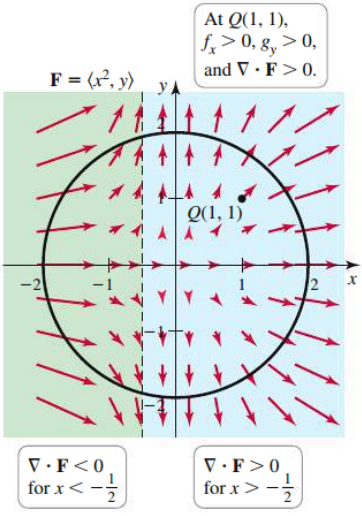
\includegraphics[width=0.75\linewidth]{images/briggs_17_05/fig17_39}
    \end{flushright}
  \end{minipage}
  \pagebreak

  \noindent
  \textbf{Curl:}

  \[\grad\times\mathbf F=
      \begin{vmatrix}
        \bfi& \bfj& \bfk\\
        \frac{\partial}{\partial x}& \frac{\partial}{\partial y}& \frac{\partial}{\partial z}\\
        f& g& h
      \end{vmatrix}
      =\bracket{
      \frac{\partial h}{\partial y}-\frac{\partial g}{\partial z},\
      \frac{\partial f}{\partial z}-\frac{\partial h}{\partial x},\
      \frac{\partial g}{\partial x}-\frac{\partial f}{\partial y}}
    \]

  \vspace*{\stretch{1}}
  \begin{flushright}
    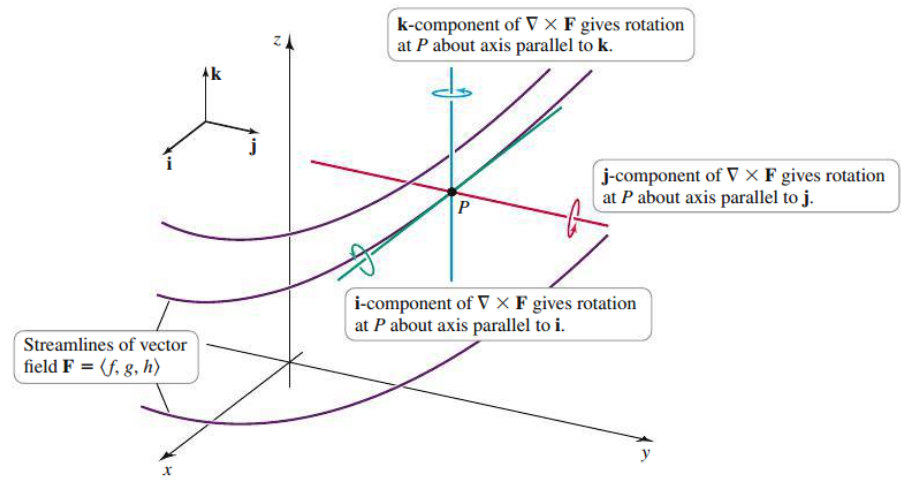
\includegraphics[width=0.8\linewidth]{images/briggs_17_05/fig17_40}
  \end{flushright}
  \vspace*{\stretch{1}}

  \begin{defn*}[Curl of a Vector Field]
    The \textbf{curl} of a vector field $\mathbf F=\bracket{f,\,g,\,h}$ that is differentiable on a region of $\bbr^3$ is
    \begin{align*}
      \grad\times\mathbf F&=\operatorname{curl} \mathbf F\\
        &=\parens{\frac{\partial h}{\partial y}-\frac{\partial g}{\partial z}}\bfi+\parens{\frac{\partial f}{\partial z}-\frac{\partial h}{\partial x}}\bfj+\parens{\frac{\partial g}{\partial x}-\frac{\partial f}{\partial y}}\bfk
    \end{align*}
    If $\grad\times\mathbf F=\bfO$, the vector field is \textbf{irrotational}.
  \end{defn*}
  \pagebreak

  \noindent
  \textbf{Curl of a General Rotation Vector Field}

  Let $\mathbf F=\veca\times\vecr$, where $\veca=\bracket{a_1, a_2, a_3}$. Then
  \vspace*{\stretch{1}}
  \begin{align*}
    \grad\cdot\mathbf F&=0&
    \grad\times\mathbf F&=2\veca
  \end{align*}

  \vspace*{\stretch{1}}
  \begin{center}
    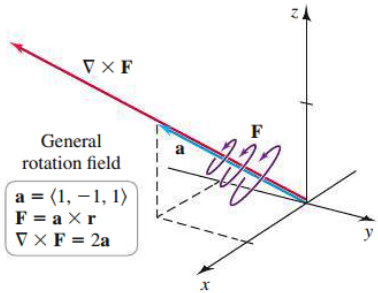
\includegraphics[width=0.5\linewidth]{images/briggs_17_05/fig17_41}
  \end{center}
  \vspace*{\stretch{1}}

  \begin{thmBox*}[General Rotation Vector Field]
    The \textbf{general rotation vector field} is $\mathbf F=\veca\times\vecr$, when the nonzero constant vector $\mathbf a=\bracket{a_1,\,a_2,\,a_3}$ is the axis of rotation and $\vecr=\bracket{x,\,y,\,z}$. For all nonzero choices of $a$, $\abs{\grad\times\mathbf F}=2\abs{\veca}$ and $\grad\cdot\mathbf F=0$. If $\mathbf F$ is a vector field, then the constant angular speed of the field is
      \[\omega =\abs{\veca}=\frac{1}{2}\abs{\grad\times\mathbf F}.\]
  \end{thmBox*}
  \pagebreak

  \begin{ex*}
    Compute the curl of the rotation field $\mathbf F=\veca\times\vecr$, where $\veca=\bracket{-3,\,2,\,1}$ and $\vecr=\bracket{x,\,y,\,z}$. What are the direction and magnitude of the curl?
  \end{ex*}
  \vspace*{\stretch{1}}
  \pagebreak

  \noindent
  \textbf{Properties of Divergence and Curl:}
  \begin{center}
    \renewcommand{\arraystretch}{1.25}
    \begin{tabular}{@{}R@{\ =\ }L@{\hspace*{30pt}}R@{\ =\ }L@{}}
      \multicolumn{2}{l}{\textbf{Divergence Properties}}&
      \multicolumn{2}{c}{\textbf{Curl Properties}}\\
      \grad\cdot\parens{\mathbf F+\mathbf G}&\grad\cdot\mathbf F+\grad\cdot\mathbf G& 
      \grad\times\parens{\mathbf F+\mathbf G}&\parens{\grad\times\mathbf F}+\parens{\grad\times\mathbf G}\\
      %
      \grad\cdot\parens{c\mathbf F}&c\parens{\grad\cdot\mathbf F}& 
      \grad\times\parens{c\mathbf F}&c\parens{\grad\times\mathbf F}
    \end{tabular}
  \end{center}
  \vspace*{\stretch{1}}

  \begin{thmBox*}[Theorem 17.11: Curl of a Conservative Vector Field]
    Suppose $\mathbf F$ is a conservative vector field on an open region $D$ of $\bbr^3$. Let $\mathbf F=\grad \varphi$, where $\varphi$ is a potential function with continuous second partial derivatives on $D$. Then $\grad\times\mathbf F=\grad\times\grad_\varphi=\bfO$: The curl of the gradient is the zero vector and $\mathbf F$ is irrotational.
  \end{thmBox*}
  
%  \vspace*{\stretch{0.25}}
  \begin{proof}
    \[\grad\times\mathbf F=\grad\times\varphi=
      \begin{vmatrix}
        \bfi& \bfj& \bfk\\
        \dfrac{\partial}{\partial x}& \dfrac{\partial}{\partial y}& \dfrac{\partial}{\partial z}\\
        \varphi_x& \varphi_y& \varphi_z
      \end{vmatrix}
      =\bracket{
        \varphi_{zy}-\varphi_{yz},\,
        \varphi_{xz}-\varphi_{zx},\,
        \varphi_{yx}-\varphi_{xy}}
      =\bfO
    \]
  \end{proof}
  \vspace*{\stretch{1}}

  \begin{thmBox*}[Theorem 17.12: Divergence of the Curl]
    Suppose $\mathbf F=\bracket{f,\,g,\,h}$, where $f$, $g$, and $h$ have continuous second partial derivatives. Then $\grad\cdot\parens{\grad\times\mathbf F}=0$: The divergence of the curl is zero.
  \end{thmBox*}
  \begin{proof}
    \begin{align*}
      \grad\cdot\parens{\grad\times\mathbf F}&=
        \frac{\partial}{\partial x}\parens{\frac{\partial h}{\partial y}-\frac{\partial g}{\partial z}}+
        \frac{\partial}{\partial y}\parens{\frac{\partial f}{\partial z}-\frac{\partial h}{\partial x}}+
        \frac{\partial}{\partial z}\parens{\frac{\partial g}{\partial x}-\frac{\partial f}{\partial y}}\\[5pt]
        &=\parens{h_{yx}-h_{xy}}+\parens{g_{xz}-g_{zx}}+\parens{f_{zy}-f_{yz}}=0
    \end{align*}
  \end{proof}
  \pagebreak

  The \textbf{Laplacian}, denoted $\grad^2 u$ or $\Delta u$, arises from $\grad\cdot\grad u$:
    \[\grad\cdot\grad u=\frac{\partial }{\partial x}\frac{\partial u}{\partial x}+\frac{\partial }{\partial y}\frac{\partial u}{\partial y}+\frac{\partial }{\partial z}\frac{\partial u}{\partial z}=\frac{\partial^2 u}{\partial x^2}+\frac{\partial^2 u}{\partial y^2}+\frac{\partial^2 u}{\partial z^2}\]
  \vspace*{\stretch{0.25}}

  \begin{thmBox*}[Theorem 17.13: Product Rule for the Divergence]
    Let $u$ be a scalar-valued function that is differentiable on a region $D$ and let $\mathbf F$ be a vector field that is differentiable on $D$. Then
      \[\grad\cdot\parens{u\mathbf F}=\grad u\cdot\mathbf F+u\parens{\grad\cdot\mathbf F}.\]
  \end{thmBox*}
  \begin{ex*}
    Let $\vecr=\bracket{x,y,z}$ and let $\varphi=\frac{1}{\abs{\vecr}}$ be a potential function.
  \end{ex*}
  \begin{tasks}[after-item-skip=\stretch{1}, label=](1)
    \task 
      Find the associated gradient field $\mathbf F=\grad\parens{\frac{1}{\abs{\vecr}}}$
    \task 
      Compute $\grad\cdot\mathbf F$
  \end{tasks}
  \vspace*{\stretch{1}}
  \pagebreak

  \begin{thmBox*}[Properties of a Conservative Vector Field]
    Let $\mathbf F$ be a conservative vector field whose components have continuous second partial derivatives on an open connected region $D$ in $\bbr^3$. Then $\mathbf F$ has the following equivalent properties.
    \begin{enumerate}
      \item 
        There exists a potential function $\varphi$ such that $\mathbf F=\grad_\varphi$ (definition).
      \item 
        $\int_C \mathbf F\cdot d\vecr=\varphi(B)-\varphi(A)$ for all points $A$ and $B$ in $D$ and all piecewise smooth oriented curves $C$ in $D$ from $A$ to $B$.
      \item 
        $\oint_C \mathbf F\cdot d\vecr=0$ on all simple piecewise-smooth closed oriented curves $C$ in $D$.
      \item 
        $\grad\times\mathbf F=\bfO$ at all points of $D$.
    \end{enumerate}
  \end{thmBox*}

  \pagebreak
  
\end{document}